\documentclass[a4paper,12pt]{extarticle}
\usepackage[utf8x]{inputenc}
\usepackage[T1,T2A]{fontenc}
\usepackage[russian]{babel}
\usepackage{hyperref}
\usepackage{indentfirst}
\usepackage{listings}
\usepackage{color}
\usepackage{here}
\usepackage{array}
\usepackage{multirow}
\usepackage{graphicx}

\usepackage{amsmath}

\usepackage{caption}
\renewcommand{\lstlistingname}{Программа} % заголовок листингов кода

\bibliographystyle{ugost2008ls}

\usepackage{listings}
\lstset{ %
extendedchars=\true,
keepspaces=true,
language=C,						% choose the language of the code
basicstyle=\footnotesize,		% the size of the fonts that are used for the code
numbers=left,					% where to put the line-numbers
numberstyle=\footnotesize,		% the size of the fonts that are used for the line-numbers
stepnumber=1,					% the step between two line-numbers. If it is 1 each line will be numbered
numbersep=5pt,					% how far the line-numbers are from the code
backgroundcolor=\color{white},	% choose the background color. You must add \usepackage{color}
showspaces=false				% show spaces adding particular underscores
showstringspaces=false,			% underline spaces within strings
showtabs=false,					% show tabs within strings adding particular underscores
frame=single,           		% adds a frame around the code
tabsize=2,						% sets default tabsize to 2 spaces
captionpos=t,					% sets the caption-position to top
breaklines=true,				% sets automatic line breaking
breakatwhitespace=false,		% sets if automatic breaks should only happen at whitespace
escapeinside={\%*}{*)},			% if you want to add a comment within your code
postbreak=\raisebox{0ex}[0ex][0ex]{\ensuremath{\color{red}\hookrightarrow\space}},
texcl=true,
inputpath=listings,                     % директория с листингами
}

\usepackage[left=2cm,right=2cm,
top=2cm,bottom=2cm,bindingoffset=0cm]{geometry}

%% Нумерация картинок по секциям
\usepackage{chngcntr}
\counterwithin{figure}{section}
\counterwithin{table}{section}

%%Точки нумерации заголовков
\usepackage{titlesec}
\titlelabel{\thetitle.\quad}
\usepackage[dotinlabels]{titletoc}

%% Оформления подписи рисунка
\addto\captionsrussian{\renewcommand{\figurename}{Рисунок}}
\captionsetup[figure]{labelsep = period}

%% Подпись таблицы
\DeclareCaptionFormat{hfillstart}{\hfill#1#2#3\par}
\captionsetup[table]{format=hfillstart,labelsep=newline,justification=centering,skip=-10pt,textfont=bf}

%% Путь к каталогу с рисунками
\graphicspath{{fig/}}


\setcounter{tocdepth}{3}

\begin{document}	% начало документа

% Титульная страница
\begin{titlepage}	% начало титульной страницы

	\begin{center}		% выравнивание по центру

		\large Санкт-Петербургский Политехнический Университет Петра Великого\\
		\large Институт компьютерных наук и технологий \\
		\large Кафедра компьютерных систем и программных технологий\\[6cm]
		% название института, затем отступ 6см
		
		\huge Телекоммуникационные технологии\\[0.5cm] % название работы, затем отступ 0,5см
		\large Отчет по лабораторной работе №4\\[0.1cm]
		\large Аналоговая модуляция\\[5cm]

	\end{center}


	\begin{flushright} % выравнивание по правому краю
		\begin{minipage}{0.25\textwidth} % врезка в половину ширины текста
			\begin{flushleft} % выровнять её содержимое по левому краю

				\large\textbf{Работу выполнил:}\\
				\large Соболь В.О.\\
				\large {Группа:} 33501/4\\
				
				\large \textbf{Преподаватель:}\\
				\large Богач Н.В.

			\end{flushleft}
		\end{minipage}
	\end{flushright}
	
	\vfill % заполнить всё доступное ниже пространство

	\begin{center}
	\large Санкт-Петербург\\
	\large \the\year % вывести дату
	\end{center} % закончить выравнивание по центру

\thispagestyle{empty} % не нумеровать страницу
\end{titlepage} % конец титульной страницы

\vfill % заполнить всё доступное ниже пространство

% Содержание
% Содержание
\renewcommand\contentsname{\centerline{Содержание}}
\tableofcontents
\newpage




\section{Цель работы}
Изучение амплитудной модуляции и демодуляции сигнала.

\section{Постановка задачи}
\begin{enumerate}
\item сгенерировать однотональный низкочастотный сигнал
\item выполнить амплитудную модуляцию этого сигнала
\item выполнить модуляцию с подавлением несущей
\item выполнить однополосную модуляцию
\item для всех типов модуляции осуществить синхронное детектирование
\item рассмотреть спектры сигналов после модуляции и после детектирования
\item рассчитать КПД модуляции
\end{enumerate}

\section{Теоретическая информация}

\subsection{Модуляция}
Модуляция --- это перенос спектра сигналов из низкочастотной области на заданную частоту. 
Это применяется для передачи сигнала в заданном частотном диапазоне.
Для модулирующего (исходного) сигнала $ S(t) $ в канале связи для передачи формируется  вспомогательный периодический высокочастотный сигнал $u(t)=f(t, [a_1,   a_2,   ...   a_m])$. Параметры $a_i$ определяют форму сигнала. 
При модуляции исходный сигнал $S(t)$ переносят на один из параметров $a_i$, форма сигнала $u(t)$ (несущей) изменяется и 
служит для переноса информации, содержащейся в сигнале $S(t)$. Обратная операция выделения сигнала $S(t)$ из 
модулированного сигнала $u(t)$ называется демодуляция.

\subsection{Однотональный сигнал}

Для генерации гармонического сигнала можно воспользоваться формулой\\ $signal = A*cos(2*\pi * f*t + \varphi)$,
 где $ A $ --- амплитуда сигнала, $f$ --- частота, $t$ --- вектор отсчетов времени, $\varphi$ --- смещение по фазе.

\subsection{Типы модуляции}
\subsubsection{Амплитудная модуляция}
Формула амплитудной модуляции имеет вид: 
\begin{equation}
	u(t) = (1 + M U_m cos(\Omega t)) cos(\omega_0 t + \varphi _0)
\end{equation}
Спектр сигнала с амплитудной модуляцией показан на рис.\ref{pic:spec_an_mod_theor}.
На графике $\omega_0$ --- частота несущей, $\Omega$ --- частота модуляции.
\begin{figure}[H]
	\begin{center}
		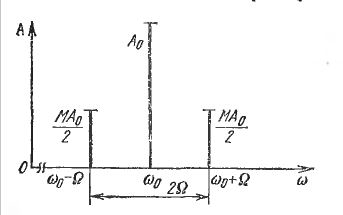
\includegraphics[scale=0.7]{spec_an_mod_theor}
		\caption{Спектр амплитудно-модулированного сигнала} 
		\label{pic:spec_an_mod_theor} % название для ссылок внутри кода
	\end{center}
\end{figure}

Амплитудная модуляция имеет низкий КПД и применяется очень редко.

\subsubsection{Амплитудная модуляция с подавлением несущей}
Основная мощность АМ сигнала приходится на несущую частоту. При АМ с подавлением несущей производится перемножение двух сигналов – модулирующего и несущего. В результате несущая частота подавляется и КПД модуляции становится 100\%.
Формула такой модуляции:
\begin{equation}
	u(t) = M U_m cos(\Omega t) cos(\omega_0 t + \varphi _0)
\end{equation}

Спектр сигнала с амплитудной модуляцией с подавлением несущей представлен на Рис.\ref{pic:spec_an_mod_carrier_theor}:
На графике $\omega_0$ --- частота несущей, $\Omega$ --- частота модуляции. Как видно в спектре
отсутствует несущая частота. 

\begin{figure}[H]
	\begin{center}
		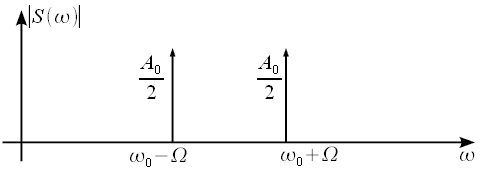
\includegraphics[scale=0.7]{spec_an_mod_carrier_theor}
		\caption{Спектр амплитудно модулированного сигнала с подавлением несущей} 
		\label{pic:spec_an_mod_carrier_theor} % название для ссылок внутри кода
	\end{center}
\end{figure}

\subsubsection{Однополосная модуляция}
При идентичности информации в группах верхних и нижних боковых частот нет необходимости в их одновременной передаче. 
Можно удалить одну из боковых частот и получить сигнал с одной боковой полосой (ОБП).
Функция сигнала с ОБП имеет вид:
 \begin{equation}
	u(t) = U_m cos(\Omega t) cos(\omega_0 t + \varphi _0) + \frac{U_m}{2} \sum_{n=1}^{N}  M_n cos((\omega_0 + \Omega_n) t + \varphi _0 + \Phi _n)
\end{equation}

Форма ОБП сигнала похожа на форму сигнала с  АМ, но ее огибающая имеет меньшую амплитуду. 
Для демодуляции ОБП сигнала может использоваться как двухполупериодное, так и синхронное детектирование, со всеми особенностями, присущими этим методам. 
Результаты демодуляции отличаются от демодуляции АМ сигналов только меньшей амплитудой выходных сигналов.

Спектр однополосно-модулированного сигнала представлен на рис.\ref{pic:spec_an_mod_singleband_theor}:
\begin{figure}[H]
	\begin{center}
		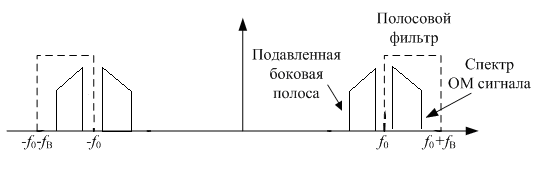
\includegraphics[scale=0.7]{spec_an_mod_singleband_theor}
		\caption{Спектр однополосно-модулированного сигнала} 
		\label{pic:spec_an_mod_singleband_theor} % название для ссылок внутри кода
	\end{center}
\end{figure}

\subsubsection{Демодуляция с помощью синхронного детектирования}
При синхронном детектировании модулированный сигнал умножается на опорное колебание с частотой несущего колебания:
 \begin{equation}
	y(t) = U(t) cos(\omega_0 t) cos(\omega_0 t) = \frac{U(t)}{2} (1 + cos(2\omega_0 t))
\end{equation}
Сигнал разделяется на два слагаемых, первое из которых повторяет исходный модулирующий сигнал, а второе повторяет модулированный сигнал на удвоенной несущей частоте 2$\omega_0$. 

Амплитудный спектр сигналов после демодуляции однозначно соотносится со спектром входного модулированного сигнала: 
амплитуды гармоник модулированного сигнала на частоте 2$\omega_0$ в два раза меньше амплитуд входного сигнала,
 постоянная составляющая равна амплитуде несущей частоты $\omega_0$ и не зависит от глубины модуляции, амплитуда
  информационного демодулированного сигнала в два раза меньше амплитуды исходного модулирующего сигнала. 

Особенностью синхронного детектирования является независимость от глубины модуляции,
 т.е. коэффициент модуляции сигнала может быть больше единицы. 
 При синхронном детектировании требуется точное совпадение фаз и частот 
 опорного колебания демодулятора и несущей гармоники АМ сигнала.

\subsubsection{КПД модуляции}
КПД амплитудной модуляции зависит от коэффициента модуляции и может быть рассчитано по следующей формуле:
 \begin{equation}
	\eta (t) =\frac{ U_m^2(t) M^2}{4 P_U}  = \frac{M^2}{2 + M^2} 
\end{equation}



\section{Ход работы}
Код, написанный для исследования представлен в листинге~\ref{code:code_1}.

\subsection{Генерация однотонального сигнала}
Для получения гармонического сигнала используется функция $s(t) = A*cos(2*\pi * f*t + \varphi)$.
Сгенерированный однотональный сигнал представлен на рис.~\ref{pic:signal_one_tone}.
\begin{figure}[H]
	\begin{center}
		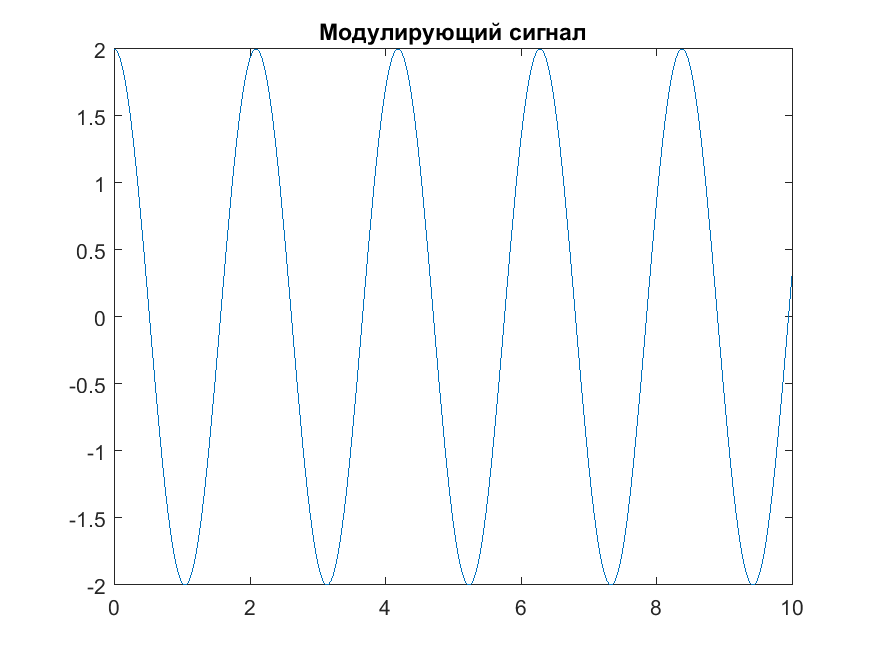
\includegraphics[scale=0.7]{signal_one_tone}
		\caption{Однотональный гармонический сигнал}
		\label{pic:signal_one_tone} % название для ссылок внутри кода
	\end{center}
\end{figure}
Спектр однотонального сигнала показан на рис.~\ref{pic:signal_one_tone_spec}.
\begin{figure}[H]
	\begin{center}
		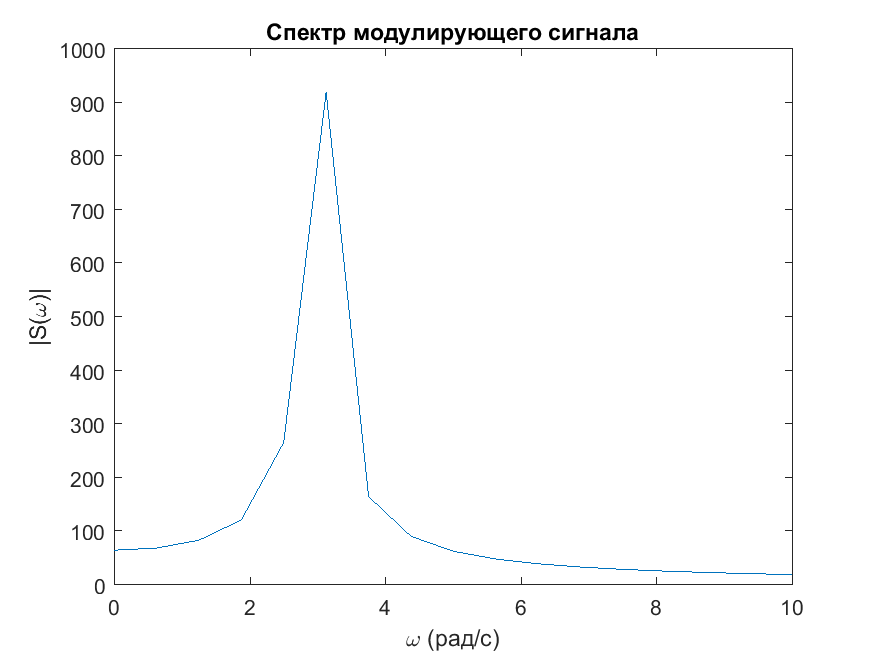
\includegraphics[scale=0.7]{signal_one_tone_spec}
		\caption{Спектр однотонального гармонического сигнала}
		\label{pic:signal_one_tone_spec} % название для ссылок внутри кода
	\end{center}
\end{figure}

\subsection{Амплитудная модуляция}
Для сгенерированного однотонального сигнала получим амплитудную модуляцию с различными
коэффициентами модуляции $ M $ (соотношением амплитуды модулирующего сигнала и амплитуды несущей).
Так же для каждого модулированного сигнала построим спектр. 
Кроме гармоники информационного сигнала в спектре видно две гармоники несущего сигнала по бокам.

\begin{enumerate}
\item Коэффициент $ M = 0.2$
\begin{figure}[H]
	\begin{center}
		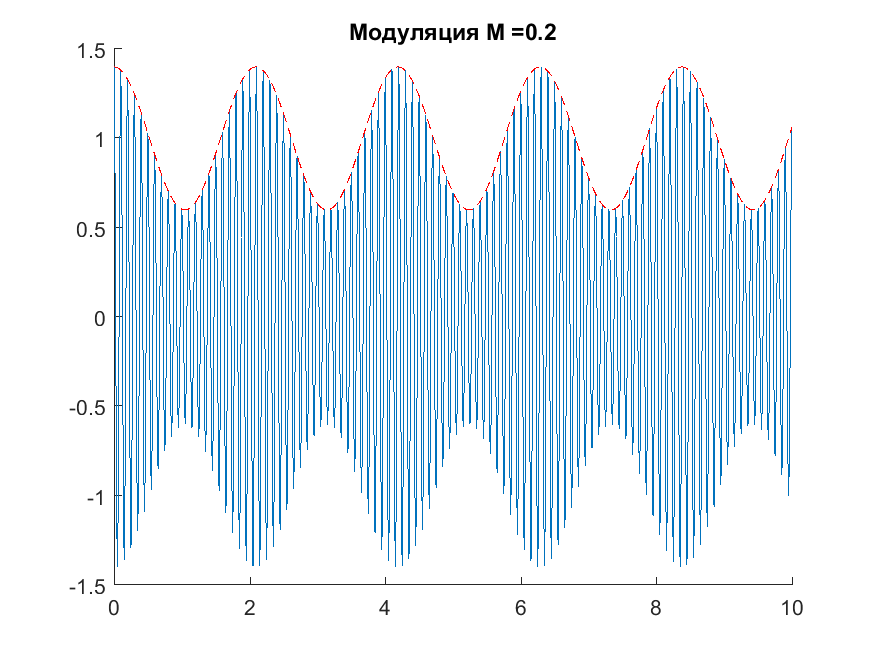
\includegraphics[scale=0.7]{mod_sig_m_0_2}
		\caption{Амплитудно-модулированный сигнал } 
		\label{pic:signal_modulated_0_5} % название для ссылок внутри кода
	\end{center}
\end{figure}

\begin{figure}[H]
	\begin{center}
		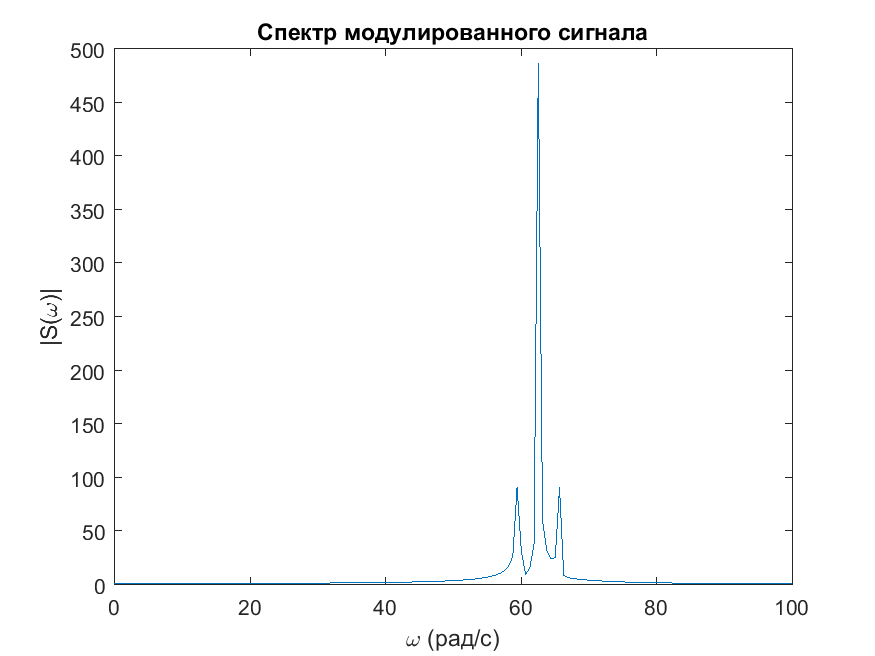
\includegraphics[scale=0.7]{mod_sig_spec_m_0_2}
		\caption{Спектр амплитудно-модулированного сигнала} 
		\label{pic:mod_sig_spec_0_5} % название для ссылок внутри кода
	\end{center}
\end{figure}


\item Коэффициент $ M = 0.5$
\begin{figure}[H]
	\begin{center}
		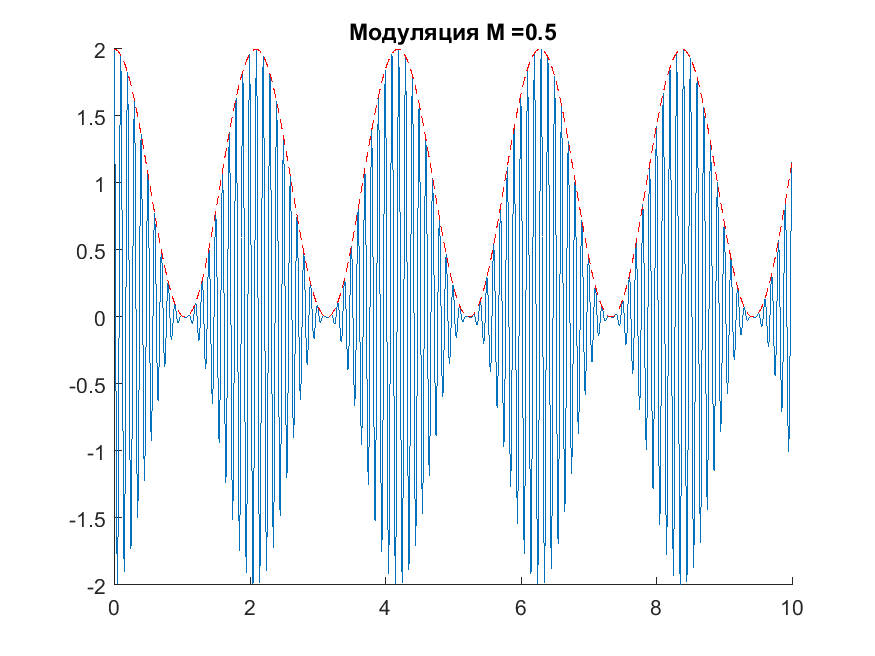
\includegraphics[scale=0.7]{mod_sig_m_0_5}
		\caption{Амплитудно-модулированный сигнал } 
		\label{pic:signal_modulated_0_2} % название для ссылок внутри кода
	\end{center}
\end{figure}
\begin{figure}[H]
	\begin{center}
		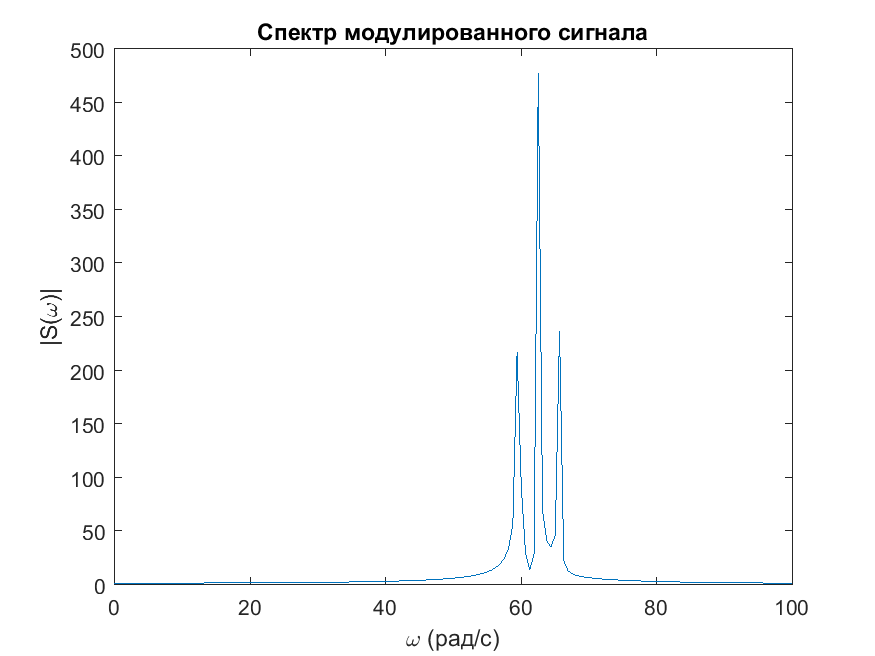
\includegraphics[scale=0.7]{mod_sig_spec_m_0_5}
		\caption{Спектр амплитудно-модулированного сигнала } 
		\label{pic:mod_sig_spec_0_2} % название для ссылок внутри кода
	\end{center}
\end{figure}

\item Коэффициент $ M = 1.0$
\begin{figure}[H]
	\begin{center}
		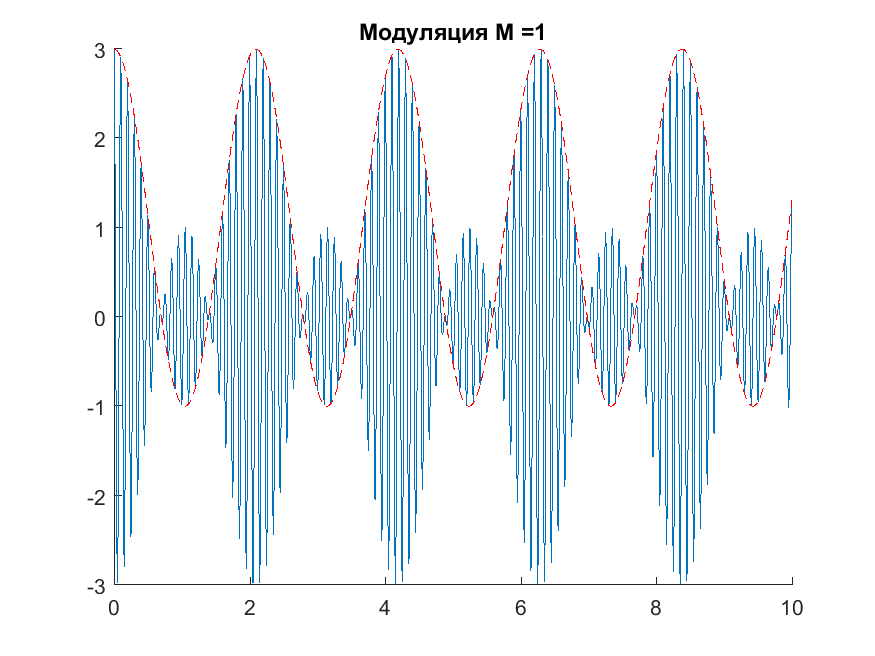
\includegraphics[scale=0.7]{mod_sig_m_1}
		\caption{Амплитудно-модулированный сигнал } 
		\label{pic:signal_modulated_1_0} % название для ссылок внутри кода
	\end{center}
\end{figure}
\begin{figure}[H]
	\begin{center}
		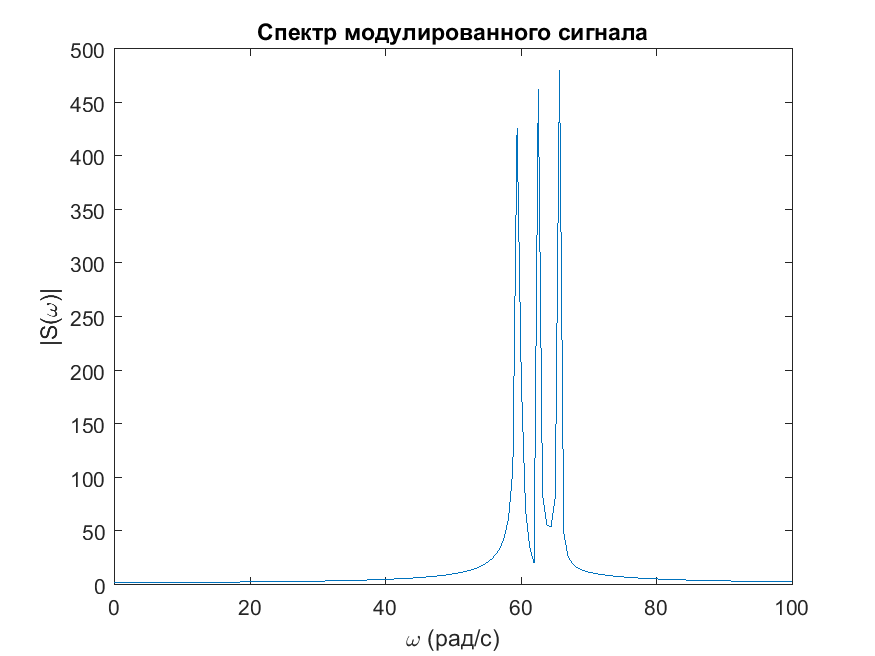
\includegraphics[scale=0.7]{mod_sig_spec_m_1}
		\caption{Спектр амплитудно-модулированного сигнала } 
		\label{pic:mod_sig_spec_1_0} % название для ссылок внутри кода
	\end{center}
\end{figure}

\item Коэффициент $ M = 2.0$
\begin{figure}[H]
	\begin{center}
		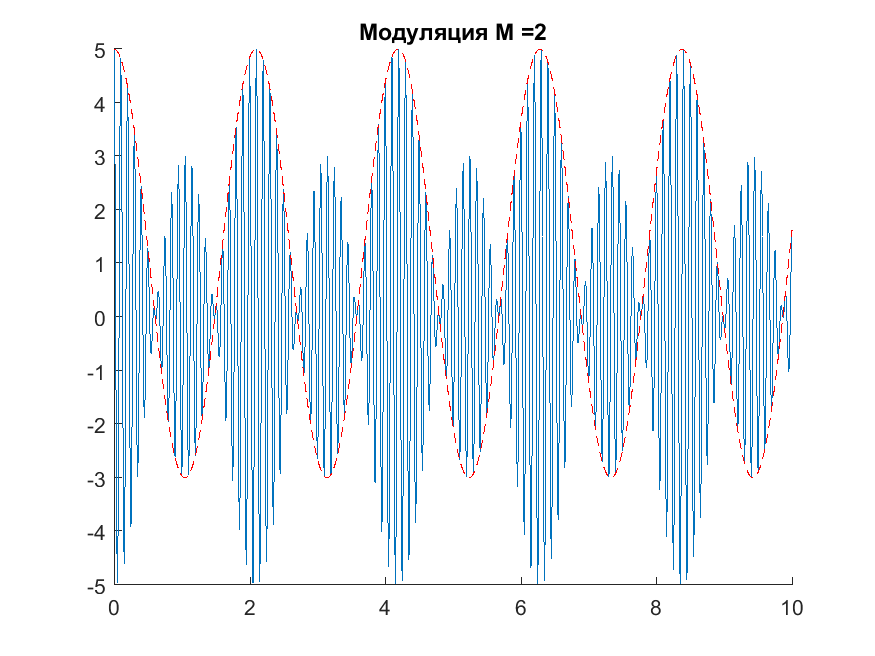
\includegraphics[scale=0.7]{mod_sig_m_2}
		\caption{Амплитудно-модулированный сигнал } 
		\label{pic:signal_modulated_2_0} % название для ссылок внутри кода
	\end{center}
\end{figure}
\begin{figure}[H]
	\begin{center}
		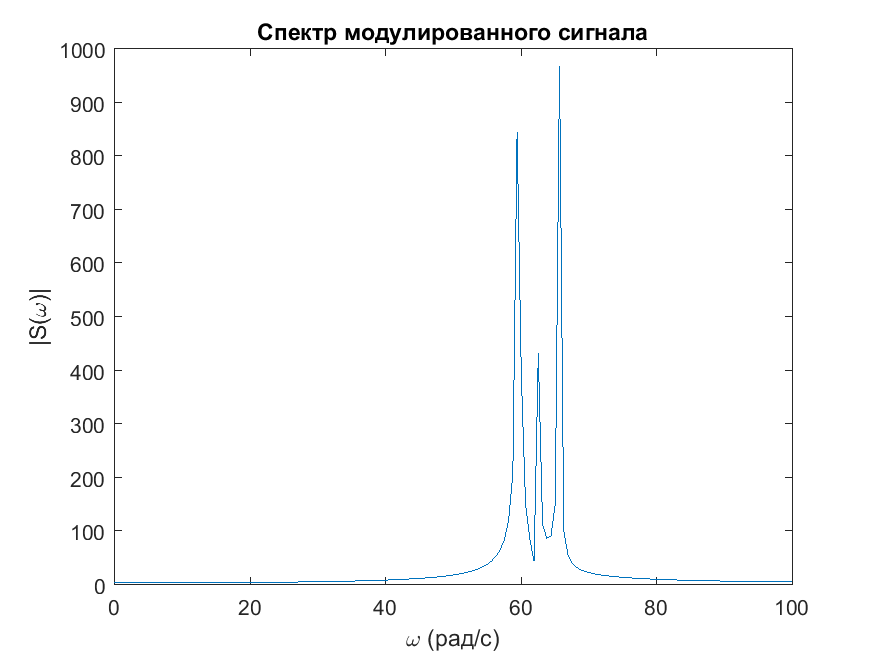
\includegraphics[scale=0.7]{mod_sig_spec_m_2}
		\caption{Спектр амплитудно-модулированного сигнала } 
		\label{pic:mod_sig_spec_2_0} % название для ссылок внутри кода
	\end{center}
\end{figure}

\item Коэффициент $ M = 5.0$
\begin{figure}[H]
	\begin{center}
		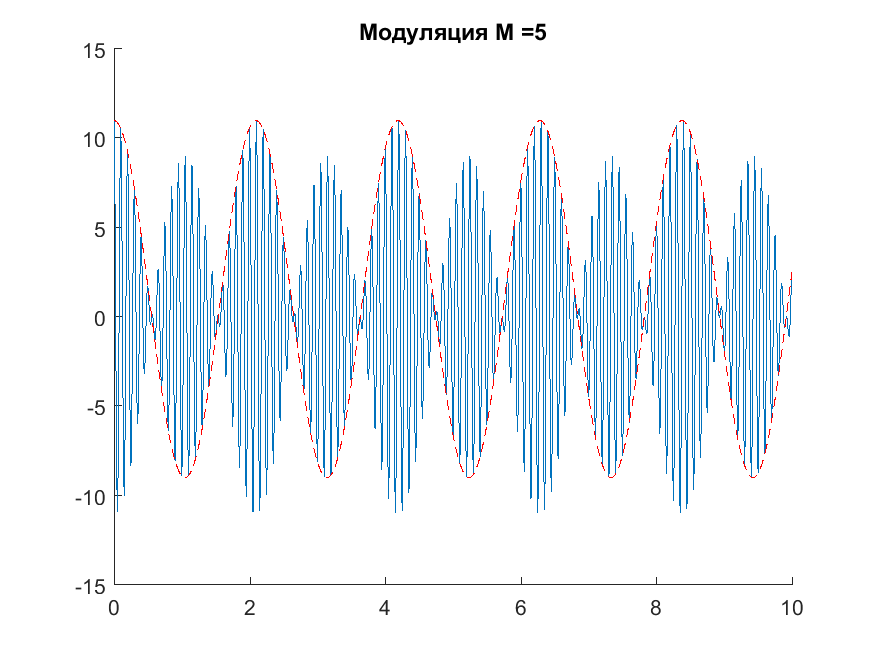
\includegraphics[scale=0.7]{mod_sig_m_5}
		\caption{Амплитудно-модулированный сигнал } 
		\label{pic:signal_modulated_2_0} % название для ссылок внутри кода
	\end{center}
\end{figure}
\begin{figure}[H]
	\begin{center}
		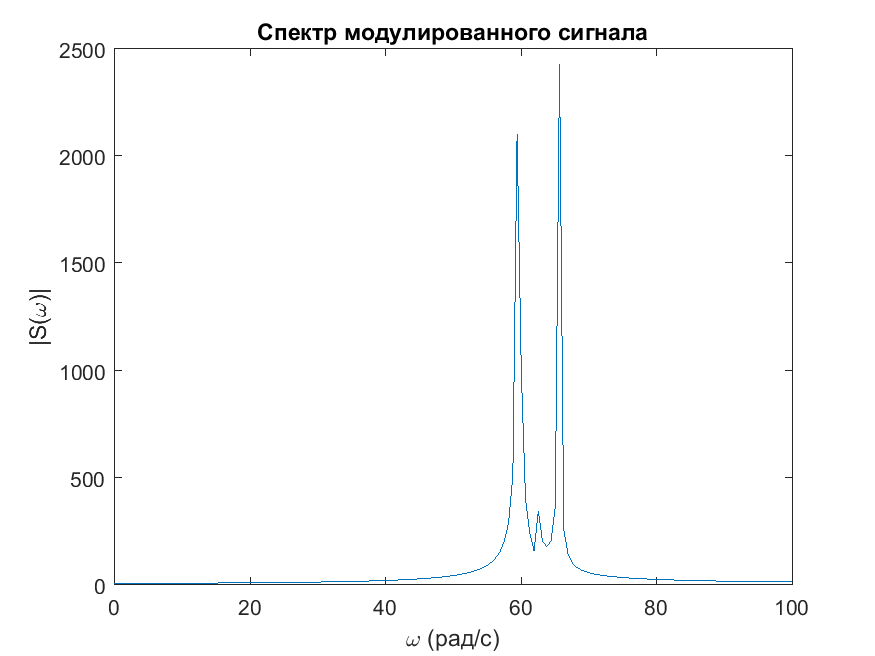
\includegraphics[scale=0.7]{mod_sig_spec_m_5}
		\caption{Спектр амплитудно-модулированного сигнала } 
		\label{pic:mod_sig_spec_2_0} % название для ссылок внутри кода
	\end{center}
\end{figure}
\end{enumerate}

При M > 1 имеем случай перемодуляции, при M = 1 - случай глубокой модуляции, а при M < 1 - обычный случай модуляции без совмещений полупериодов гармонического сигнала огибающей.

\subsection{Амплитудная модуляция с подавлением несущей}
Подавление несущей осуществляется узкополосной фильтрацией сигнала на частоте информационного.
 Сигнал с АМ с подавлением несущей представлен на рис~\ref{pic:signal_mod_carrier}.
 Спектр модулированного сигнала показан на рис.~\ref{pic:signal_mod_carrier_spec}
\begin{figure}[H]
	\begin{center}
		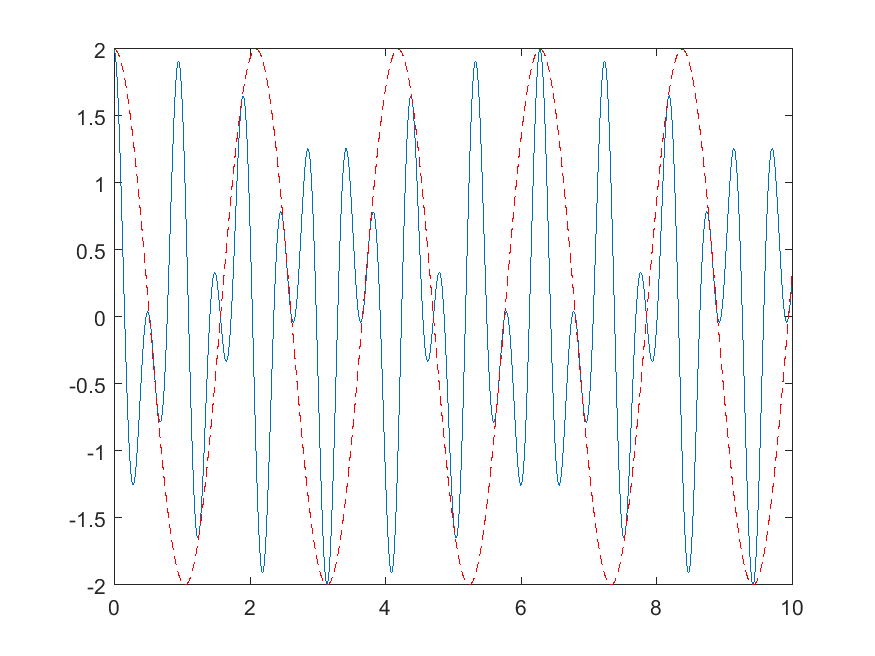
\includegraphics[scale=0.7]{sig_mod_carrier}
		\caption{Амплитудно-модулированный сигнал с подавлением несущей} 
		\label{pic:signal_mod_carrier} % название для ссылок внутри кода
	\end{center}
\end{figure}
\begin{figure}[H]
	\begin{center}
		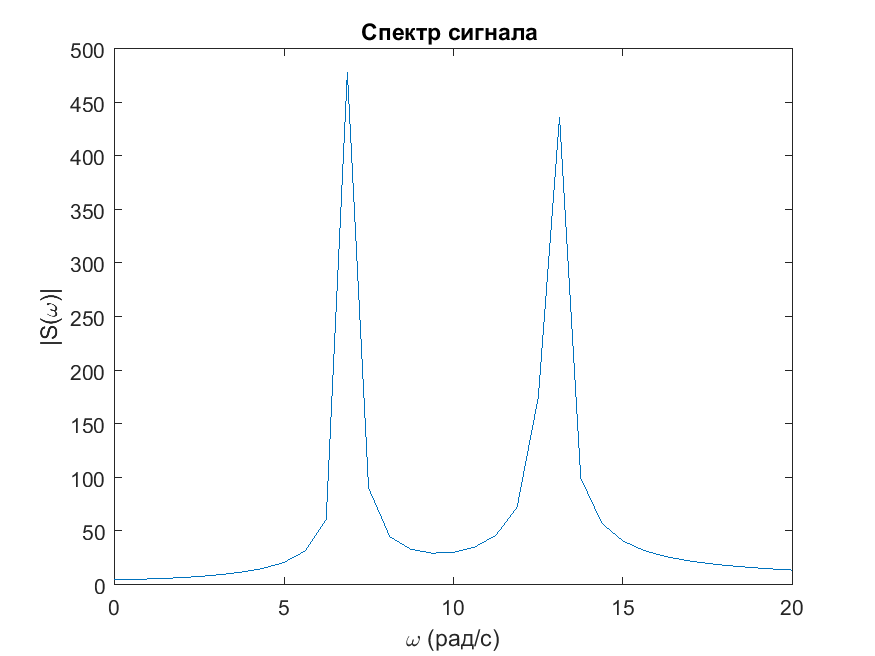
\includegraphics[scale=0.7]{sig_mod_carrier_spec}
		\caption{Спектр амплитудно-модулированного сигнала с подавлением несущей} 
		\label{pic:signal_mod_carrier_spec} % название для ссылок внутри кода
	\end{center}
\end{figure}
В спектре видно отсутствие несущей, что соответствует АМ с подавлением несущей.
Подавление несущей приводит к тому, что основная мощность сигнала (приходящаяся на несущую гармонику) фильтруется.
Демодулировать такой сигнал невозможно, поэтому применяют частичную фильтрацию, то есть сохранение амплитуды несущей гармоники ненулевой, но более низкой, чем у информационной составляющей.

\subsection{Однополосная амплитудная модуляция}
Помимо подавления несущей, можно избавиться от лишней (дублирующейся) боковой полосы спектра с помощью 
фильтра низких частот. Модулированный сигнал представлен на рис.~\ref{pic:signal_mod_singleband}.
Его спектр показан на рис.~\ref{pic:signal_mod_singleband_spec}.
\begin{figure}[H]
	\begin{center}
		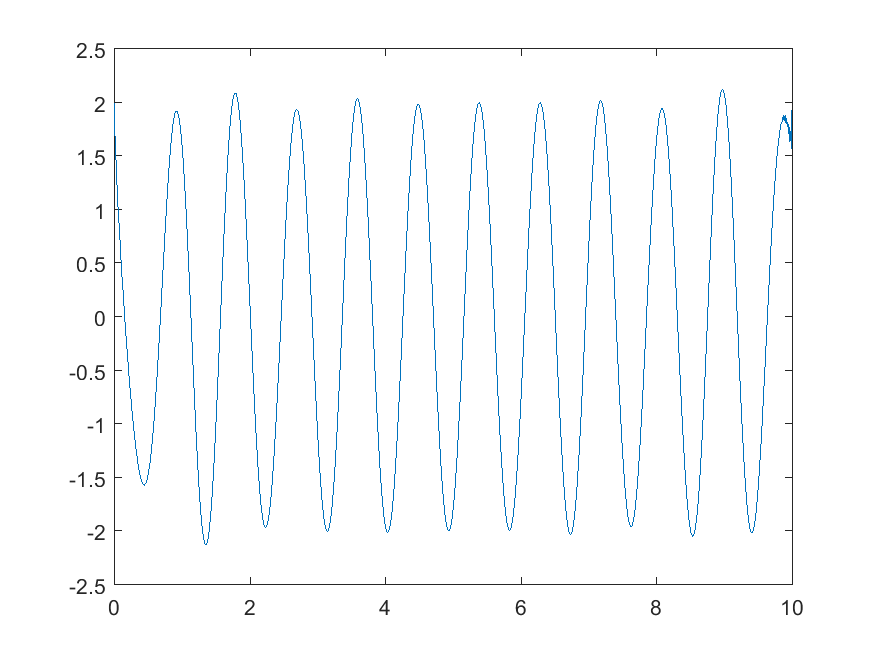
\includegraphics[scale=0.7]{sig_mod_single}
		\caption{Однополосно-модулированный сигнал} 
		\label{pic:signal_mod_singleband} % название для ссылок внутри кода
	\end{center}
\end{figure}
\begin{figure}[H]
	\begin{center}
		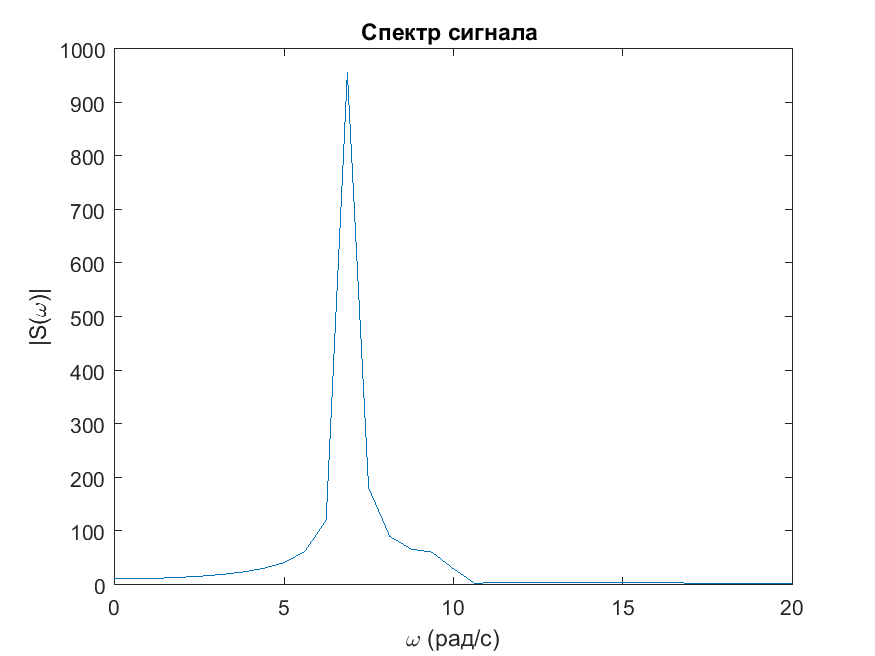
\includegraphics[scale=0.7]{sig_mod_single_spec}
		\caption{Спектр однополосно-модулированного сигнала} 
		\label{pic:signal_mod_singleband_spec} % название для ссылок внутри кода
	\end{center}
\end{figure}
Спектр содержит одну полосу, что соответствует однополосной амплитудной модуляции.

\subsection{Демодуляция с помощью синхронного детектирования}
Произведем демодуляцию модулированных сигналов с разными коэффициентами модуляции.

\begin{enumerate}
\item Коэффициент $ M = 0.2$
\begin{figure}[H]
	\begin{center}
		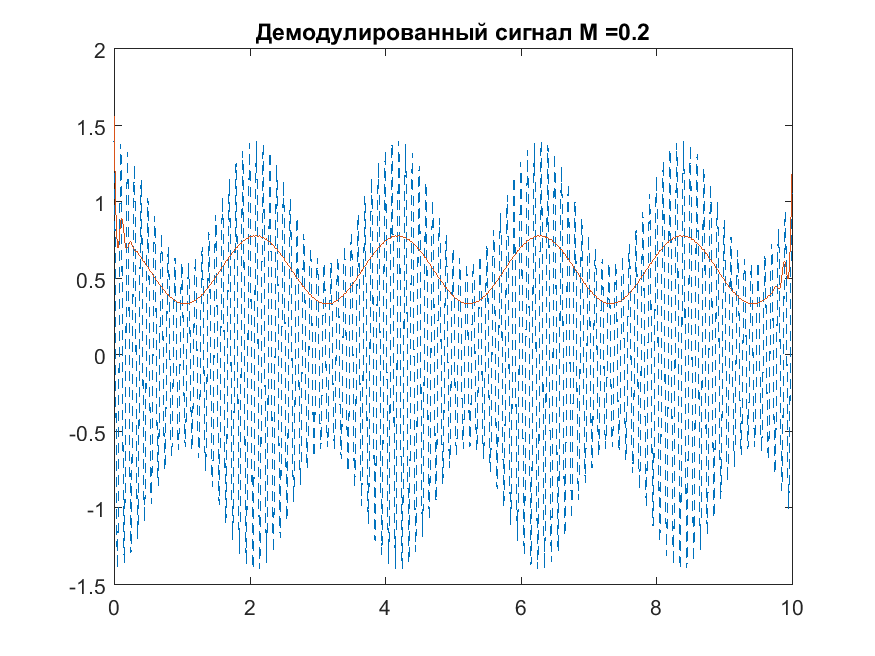
\includegraphics[scale=0.7]{demod_sig_m_0_2}
		\caption{Демодулированный сигнал } 
		\label{pic:signal_demodulated_0_5} % название для ссылок внутри кода
	\end{center}
\end{figure}

\begin{figure}[H]
	\begin{center}
		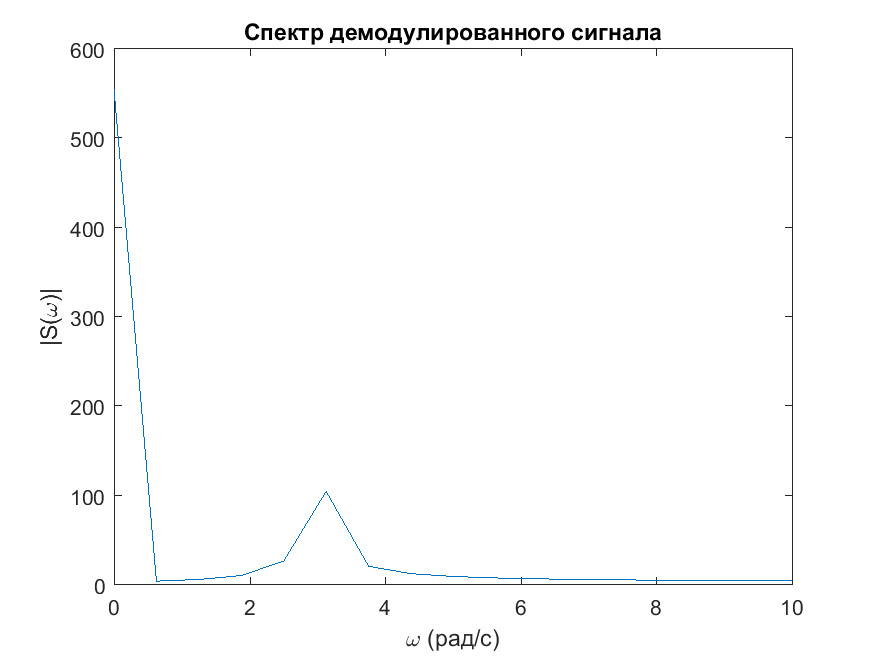
\includegraphics[scale=0.7]{demod_sig_spec_m_0_2}
		\caption{Спектр демодулированного сигнала} 
		\label{pic:demod_sig_spec_0_5} % название для ссылок внутри кода
	\end{center}
\end{figure}


\item Коэффициент $ M = 0.5$
\begin{figure}[H]
	\begin{center}
		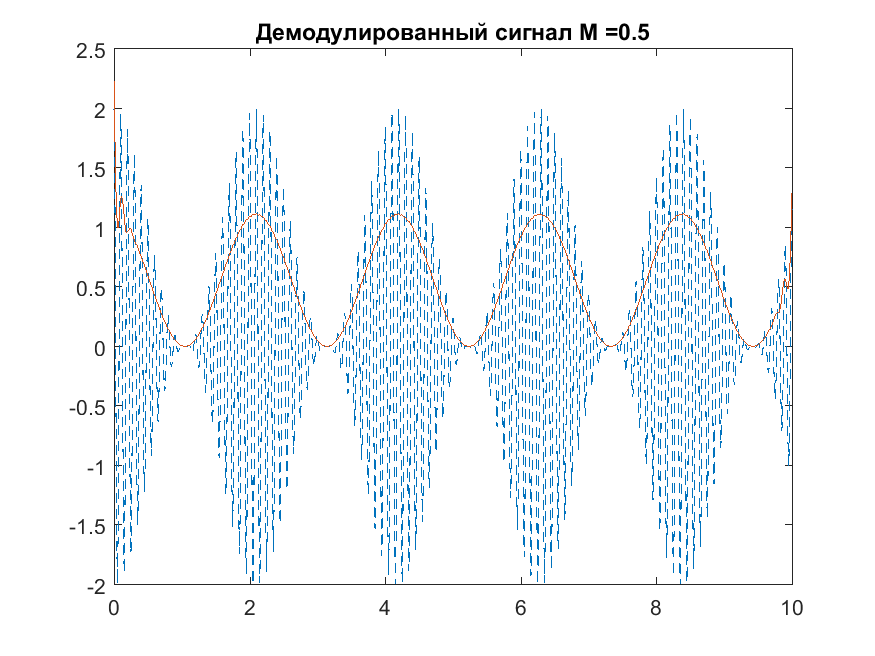
\includegraphics[scale=0.7]{demod_sig_m_0_5}
		\caption{Демодулированный сигнал } 
		\label{pic:signal_demodulated_0_2} % название для ссылок внутри кода
	\end{center}
\end{figure}
\begin{figure}[H]
	\begin{center}
		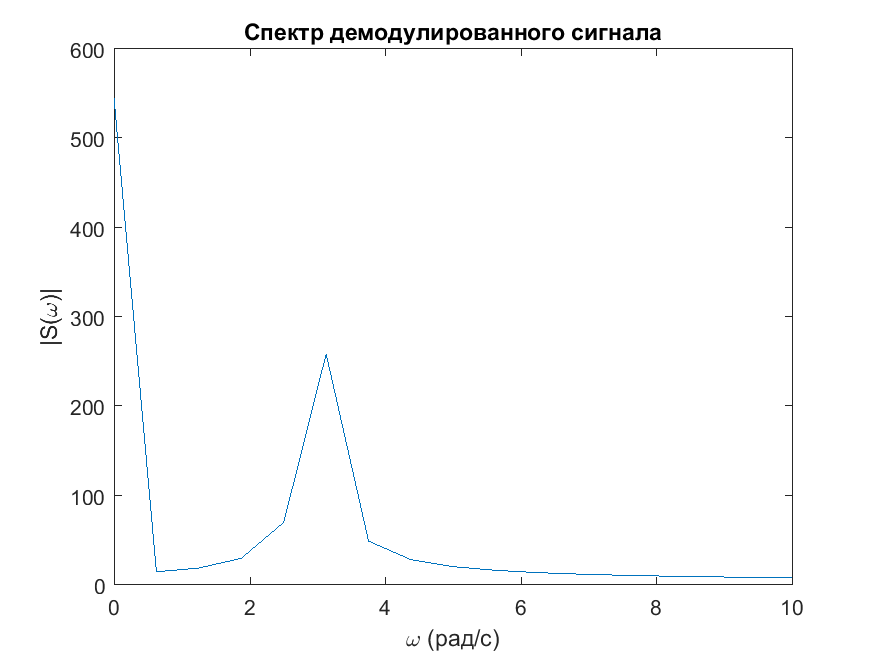
\includegraphics[scale=0.7]{demod_sig_spec_m_0_5}
		\caption{Спектр демодулированного сигнала} 
		\label{pic:demod_sig_spec_0_2} % название для ссылок внутри кода
	\end{center}
\end{figure}

\item Коэффициент $ M = 1.0$
\begin{figure}[H]
	\begin{center}
		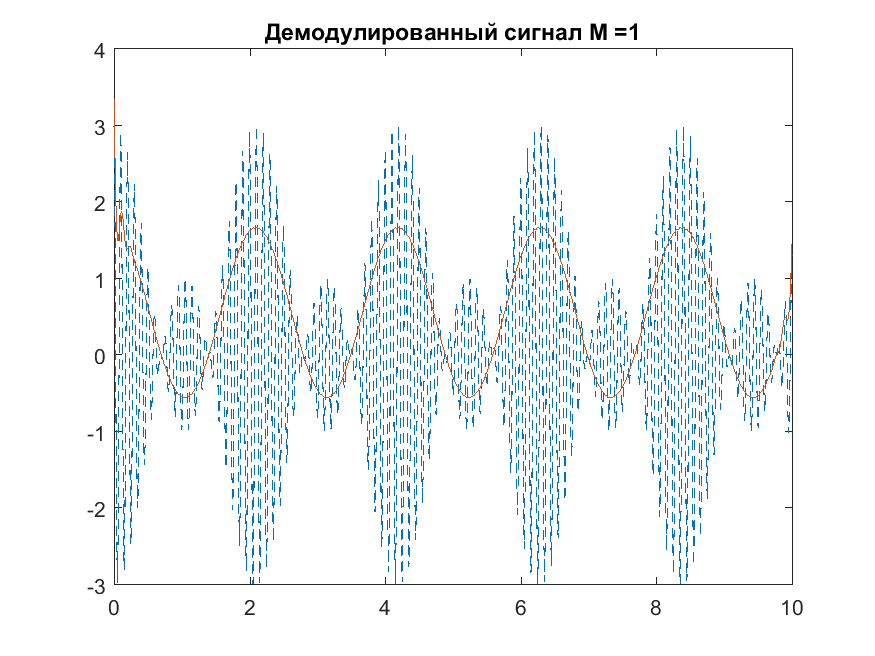
\includegraphics[scale=0.7]{demod_sig_m_1}
		\caption{Демодулированный сигнал } 
		\label{pic:signal_demodulated_1_0} % название для ссылок внутри кода
	\end{center}
\end{figure}
\begin{figure}[H]
	\begin{center}
		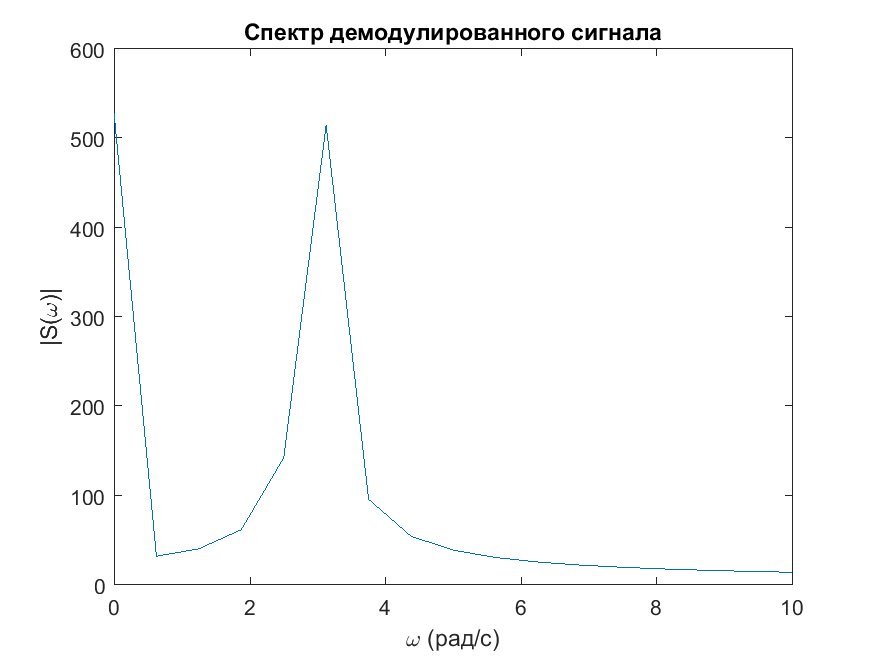
\includegraphics[scale=0.7]{demod_sig_spec_m_1}
		\caption{Спектр демодулированного сигнала} 
		\label{pic:demod_sig_spec_1_0} % название для ссылок внутри кода
	\end{center}
\end{figure}

\item Коэффициент $ M = 2.0$
\begin{figure}[H]
	\begin{center}
		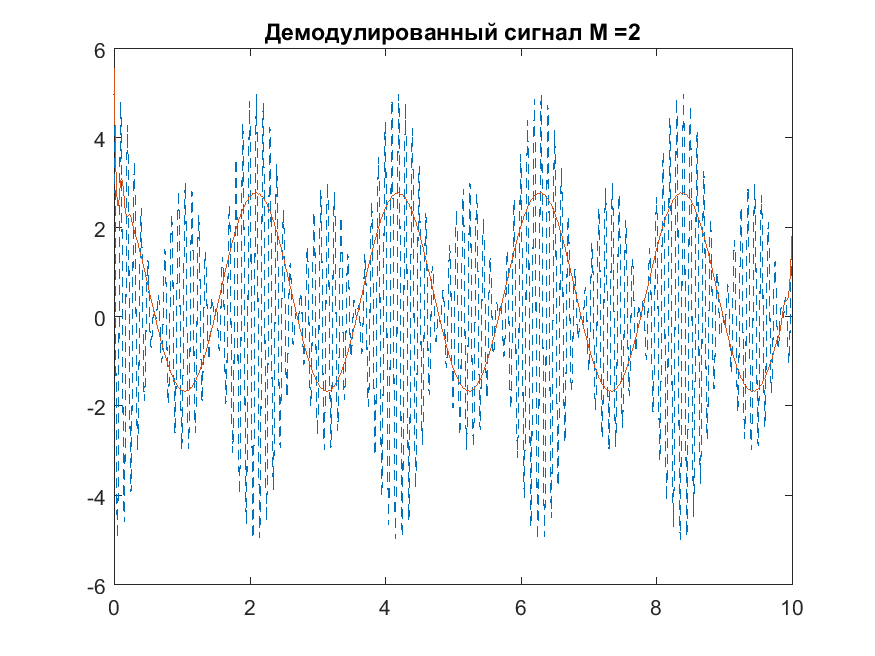
\includegraphics[scale=0.7]{demod_sig_m_2}
		\caption{Демодулированный сигнал } 
		\label{pic:signal_demodulated_2_0} % название для ссылок внутри кода
	\end{center}
\end{figure}
\begin{figure}[H]
	\begin{center}
		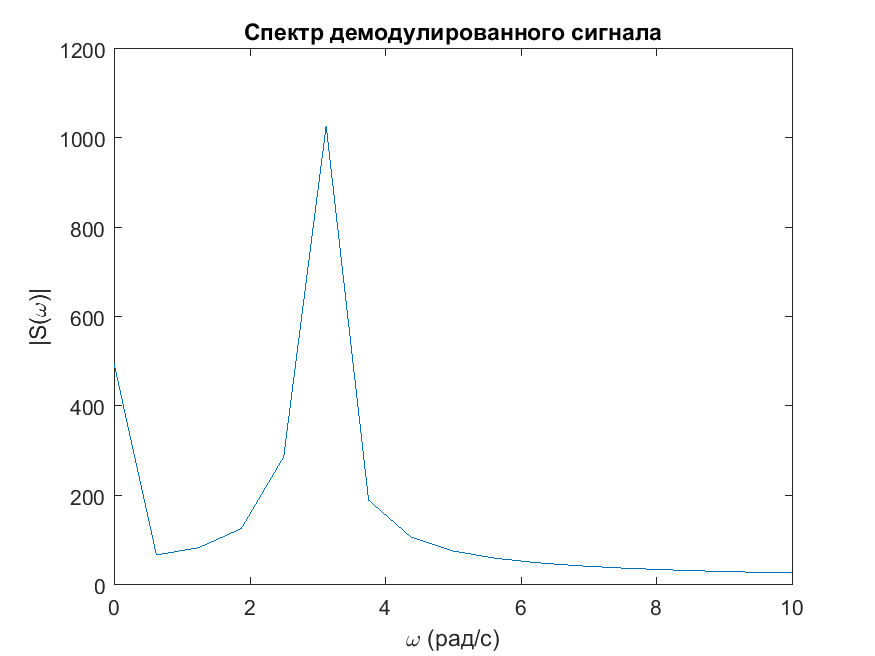
\includegraphics[scale=0.7]{demod_sig_spec_m_2}
		\caption{Спектр демодулированного сигнала} 
		\label{pic:demod_sig_spec_2_0} % название для ссылок внутри кода
	\end{center}
\end{figure}

\item Коэффициент $ M = 5.0$
\begin{figure}[H]
	\begin{center}
		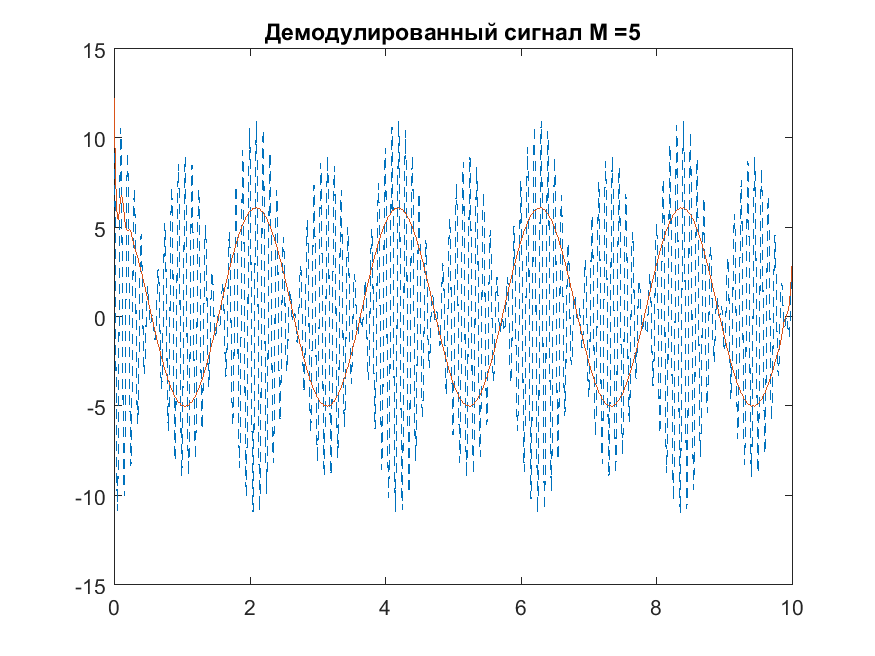
\includegraphics[scale=0.7]{demod_sig_m_5}
		\caption{Демодулированный сигнал } 
		\label{pic:signal_demodulated_2_0} % название для ссылок внутри кода
	\end{center}
\end{figure}
\begin{figure}[H]
	\begin{center}
		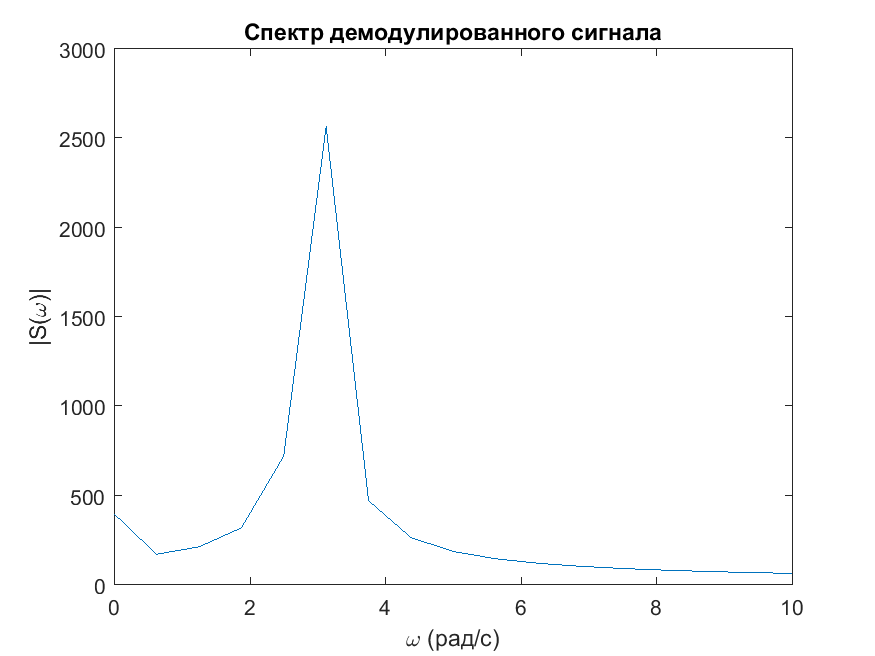
\includegraphics[scale=0.7]{demod_sig_spec_m_5}
		\caption{Спектр демодулированного сигнала} 
		\label{pic:demod_sig_spec_2_0} % название для ссылок внутри кода
	\end{center}
\end{figure}
\end{enumerate}

Как можно видеть, нелинейные искажения сигнала при демодуляции тем незначительнее, чем больше коэффициент модуляции.
В спектре демодулированного сигнала видны искажения в области низких частот, но с 
увеличением коэффициента модуляции они уменьшаются.

\subsection{КПД модуляции}
На графике (рис.~\ref{pic:Kpd_ampmod}), приведена зависимость КПД модуляции от амплитуды модулирующего сигнала
 (т.е. от коэффициента модуляции).
\begin{figure}[H]
	\begin{center}
		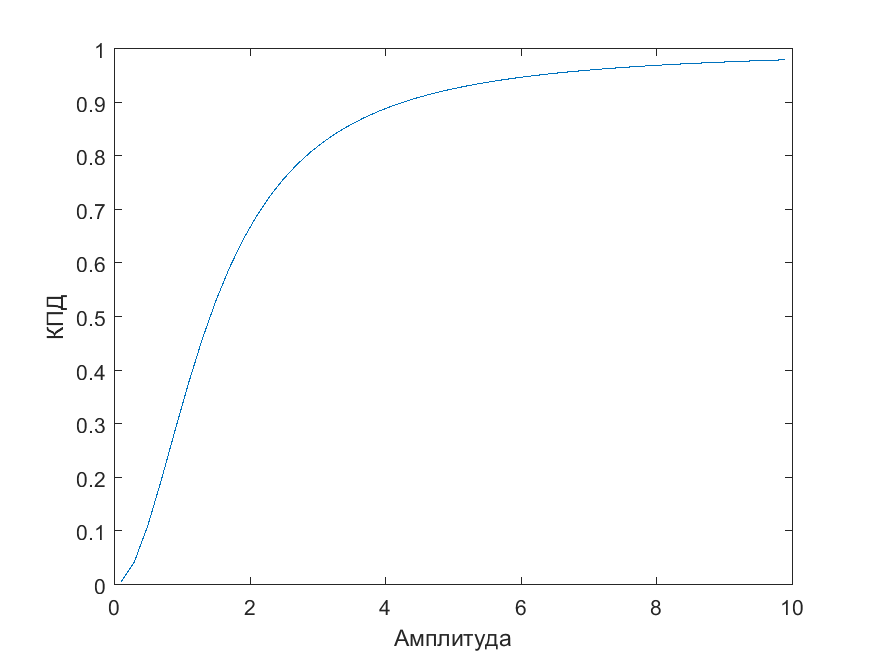
\includegraphics[scale=0.7]{kpd_plot}
		\caption{Зависимость КПД модуляции от амплитуды модулирующего сигнала} 
		\label{pic:Kpd_ampmod} % название для ссылок внутри кода
	\end{center}
\end{figure}

\section{Выводы}

В ходе этой работы нами были исследованы типы аналоговой модуляции - амплитудная, с подавлением несущей и однополосная, также исследован способ демодуляции с помощью синхронного детектирования и определена зависимость КПД модуляции от коэффициента модуляции. Также были построены спектры модулированных сигналов, их вид совпал с ожидаемым результатом для каждого типа модуляции.

По результатам работы можно сделать вывод о низкой эффективности амплитудной модуляции. 
Качество модуляции зависит от амплитуды несущего сигнала, и для обеспечения высокого качества
нужна высокая амплитуда. Из-за этого появляется необходимость использовать для передачи сигнал с 
очень большой амплитудой, что приводит к высоким потреблениям энергии. 
\section{Листинг}
\lstinputlisting[language=Matlab,
	label=code:code_1,
	caption={Код использованный для исследования},
]{lab4.m}
\end{document}
